\documentclass[../proyecto.tex]{subfiles}

\begin{document}
\chapter{Análisis del problema}
\section{WiFi}

Para poder usar una red Wi-Fi el primer paso que debe realizar un cliente es encontrar la red, para ello debe realizar un proceso de escaneo del medio para encontrar una red a la que unirse. Existen dos métodos de escaneo de redes Wi-Fi: pasivo y activo \cite{ieee80211_2016}. En el escaneo pasivo el cliente enciende el receptor y escanea en cada canal esperando que un punto de acceso se anuncie mediante un \textit{beacon frame}, el cliente almacena en un \textit{buffer} todos los \textit{bacons} recibidos para posteriormente extraer información del punto de acceso que lo emitió, este método no se considera muy eficiente. Para mejorar este proceso de descubrimiento la mayoría de dispositivos suelen utilizar el método de escaneó activo en que el cliente también analiza cada canal uno a uno pero en lugar de esperar a que la red se anuncie realiza un escaneo activo para encontrar la red, para ello envía \textit{Probe Request frames}, normalmente a la dirección broadcast (ff:ff:ff:ff:ff:ff), solicitando respuesta de un punto de acceso pudiendo indicar opcionalmente el identificador de la red (SSID) este último tipo se denomina \textit{directed probe request}, una vez emitido inicia un contador a cero y espera una respuesta, si no la recibe pasa al siguiente canal. El tiempo que espera una estación para recibir una respuesta está definido por cada fabricante pero suele rondar los 10 milisegundos, en cualquier caso, suele ser menor que el intervalo con el que los puntos de acceso emiten los \textit{beacons}.

Cuando un punto de acceso detecta un \textit{Probe Request} con el identificador de su red responde al cliente con un \textit{Probe Response frame}\\
% añadir más información sobre la respuesta del punto de acceso

En el escaneo pasivo la identidad del cliente es anónima mientras que el escaneo activo el cliente envía su dirección MAC que es un identificador único asignado por el fabricante, esto propicia que este método de descubrimiento pueda ser utilizado por terceros para detectar y registrar la presencia dispositivos en punto y tiempo concretos.\\
% contexto de que aporta al proyecto que exista este tipo de escaneo

Las tramas \textit{Probe Request frames} utilizadas en el escaneo activo son un subtipo de las tramas de tipo \textit{Management} definidas en la subcapa MAC (\textit{Medium Access Control}) del estándar IEEE 802.11, este tipo de tramas se utilizan para funciones de supervisión como puede ser unirse o salir de una red.\\

Una trama MAC está compuesta de los siguientes componentes:
\begin{enumerate}
  \item Una cabecera MAC (\textit{MAC header}).
  \item El cuerpo de la trama (\textit{Frame body}) determinado por el tipo y subtipo.
  \item Un FCS (\textit{Frame Check Sequence}) que contiene un CRC de 32 bits.
\end{enumerate}

\begin{figure}[H]
\centering
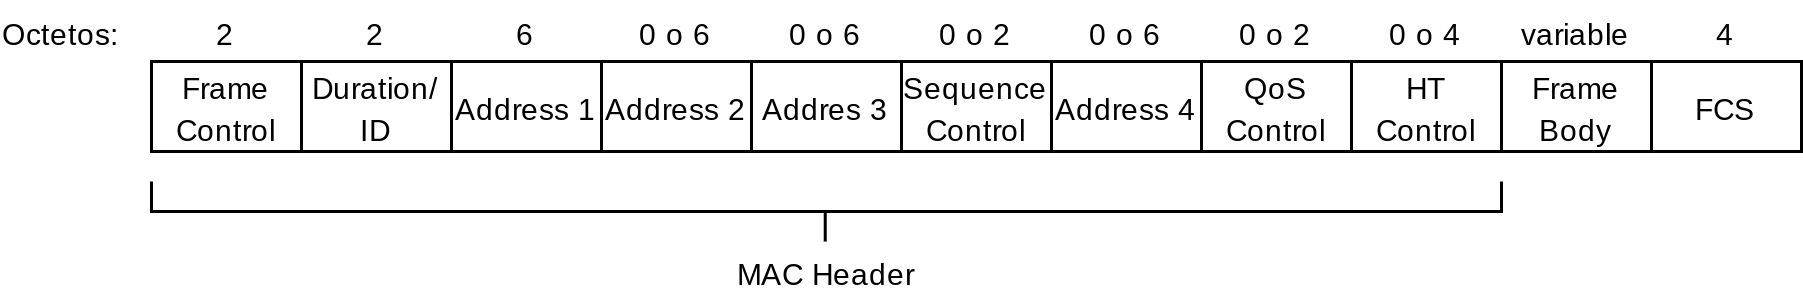
\includegraphics[scale=0.8]{analisis/mac_frame_format}
\caption{IEEE 802.11 MAC frame}
\label{fig:ieee80211_mac_frame}
\end{figure}

Los primeros tres campos (\textit{Frame Control}, \textit{Duration/ID} y \textit{Address 1}) y el último campo (\textit{FCS}) constituyen el conjunto mínimo de campos necesarios y están presentes en todas las tramas. El resto de campos están presentes solo en determinados tipos y subtipos de tramas.\\

Para el propósito de este proyecto solo necesitamos analizar la cabecera de la trama, en concreto los campos más relevantes son el \textit{Frame Control} que permitirá determinar el tipo de trama y el campo \textit{Address 2} que almacenará la dirección MAC de la estación emisora.\\

Existen dos formatos diferentes para el campo \textit{Frame Control}, este formato viene determinado por los campos \textit{Type} y \textit{Subtype}, en este caso es de interés el formato para las tramas cuyo tipo es diferente de 1 o el subtipos es diferente de 6, en cuyo caso el campo \textit{Frame Control} será como el ilustrado en la Figura \ref{fig:ieee80211_frame_control_field}

\begin{figure}[H]
\centering
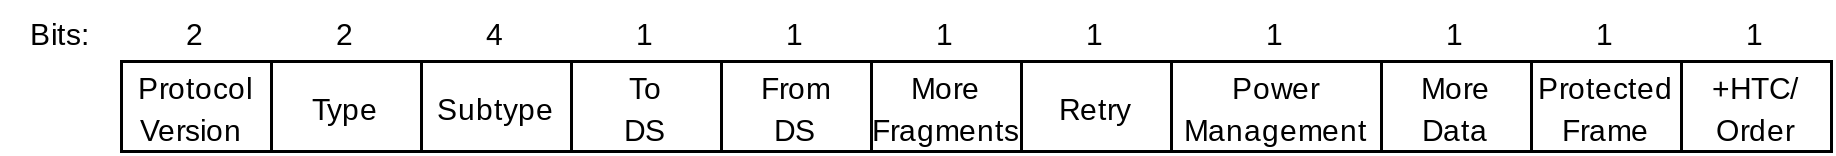
\includegraphics[scale=0.8]{analisis/frame_control_field}
\caption{IEEE 802.11 Frame Control field}
\label{fig:ieee80211_frame_control_field}
\end{figure}

El campo \textit{Type} permite determinar si se trata de una trama de tipo \textit{Management}, en la Tabla \ref{table:tipos_trama} se muestran los posibles valores que puede tomar el campo.\\

\begin{table}[h!]
\centering
\begin{tabular}{ |l|m{20em}| }
\hline
\textbf{Type} & \textbf{Descripción} \\
\hline\hline
00  & Management          \\ \hline
01  & Control  \\ \hline
10  & Data \\ \hline
11 & Extension \\ \hline
\end{tabular}
\caption{Tipos de trama}
\label{table:tipos_trama}
\end{table}

Una vez identificada la trama como tipo \textit{Management} (00) los posibles valores que puede tomar el campo \textit{Subtype} son los mostrados en la tabla \ref{table:subtipos_trama}, en concreto el valor para las tramas del subtipo \textit{Probe Request} es el 0100.

\begin{table}[h!]
\centering
\begin{tabular}{ |l|m{20em}| }
\hline
\textbf{Subtype} & \textbf{Descripción} \\
\hline\hline
0000  & Association Request  \\ \hline
0001  & Association Response \\ \hline
0010  & Reassociation Request \\ \hline
0011  & Reassociation Response \\ \hline
0100  & Probe Request \\ \hline
0101  & Probe Response \\ \hline
0110  & Timing Advertisement \\ \hline
0111  & Reserved \\ \hline
1000  & Beacon \\ \hline
1001  & ATIM \\ \hline
1010  & Disassociation \\ \hline
1011  & Authentication \\ \hline
1100  & Deauthentication \\ \hline
1101  & Action \\ \hline
1110  & Action No Ack \\ \hline
1111  & Reserved \\ \hline
\end{tabular}
\caption{Subtipos de trama para el tipo \textit{Management}}
\label{table:subtipos_trama}
\end{table}

En las tramas de tipo de tipo \textit{Management} y subtipo \textit{Probe Request} el campo \textit{Address 2} contendrá la dirección de la estación que ha emitido el \textit{Probe Request}.

\section{Bluetooth Low Energy}

\textit{Bluetooth Low Energy} (BLE) es una tecnología de red inalámbrica originalmente diseñada por Nokia bajo el nombre Wibree y adoptada después por el  el \textit{Bluetooth Special Interest Group}, empezó como parte de la especificación Core del Bluetooth 4.0 y fue puesta en el mercado en 2010. Desde el principio el propósito de su desarrollo fue diseñar un estándar de radio con el menor consumo posible, enfocado a dispositivos de bajo coste y con un ancho de banda bajo. A pesar del poco tiempo que lleva en el mercado a tenido una gran adopción debido al gran crecimiento del mercado de dispositivos móviles y \textit{wearables}.\\

% más datos sobre las posibildiades que ofrece BLE

BLE trabaja con 40 canales en la banda ISM de 2.4 GHz cada uno separado por 2MHz y define dos tipos de transmisiones: datos y \textit{advertising}. 37 de estos canales se utilizan para las conexiones de datos y los últimos tres canales (37, 38 y 39) son usados como canales de \textit{advertising} para establecer nuevas conexiones o enviar datos de difusión.

% Tipos de direcciones

BLE solo tiene un formato de paquete y dos tipos de paquetes: datos y \textit{advertising}. Un paquete de \textit{advertising} está compuesto de una cabecera, que incluye entre otros datos la dirección bluetooth del dispositivo emisor, y una carga útil de datos de hasta 31 bytes. Estos paquetes se emiten por \textit{broadcast} a un ratio de entre 20 ms y 10.24 s.

% explicación de interval y windows en el scaner


\section{Microcontrolador}

%TODO Añadir el resto de placas e introducción
Bajo coste.
Bajo consumo energético.
Reducidas dimensiones.
Conectividad bluetooth.

\noindent{\textbf{Espressif Systems SoCs}}\\
Espressif es una compañía fundada en 2008 en China y con sede en Shanghai enfocada en el desarrollo de soluciones IoT que desarrolla \textit{chipsets} y módulos WiFi y/o Bluetooth/BLE de pequeñas dimensiones con un gran rendimiento, bajo consumo y coste enfocados principalmente a dotar de conectividad a los productos de otras compañías. Son los creadores de los populares SoCs ESP8266 y ESP32 que además tener una gran penetración en el mercado de IoT han tenido un gran éxito en la comunida maker.

\noindent{\textbf{ESP8266}}\\

El ESP8266, oficialmente ESP8266EX, es un SoC WiFi de bajo coste con una pila TCP/IP lanzado al mercado en 2014 \cite{esp8266_overview}, este fue el módulo con el que Espressif comenzó a popularizarse. Se comercializa principalmente en tres formatos: SoC, módulos y módulos de desarrollo (\textit{DevKit})\\

Espressif desarrollo este SoC pensando en las necesidades de la industria del Internet of Things, como son el bajo consumo energético, un diseño compacto y la fiabilidad y durabilidad. Con una capacidad WiFI completa y autónoma puede funcionar de forma independiente o como adaptador WiFi para cualquier controlador a través de las interfaces SPI/SDIO o UART. Estas cualidades han propiciado que su utilización se haya extendido en la industria de la domótica, por ejemplo, en enchufes y bombillas inteligentes. \\

Integra un microcontrolador Tensilica L106 de 32 bits (RISC) de bajo consumo que trabaja a unos 80 MHz por defecto pudiendo alcanzar hasta 160 MHz. Además incorpora otros componentes de interfaz como SDIO, SPI, I2C, I2S, UART, PWM, conversor ADC de 10 bits y 17 GPIO. Todos estos componentes se encuentran empaquetados en tan solo 5 mm x 5 mm en un formato QFN de 32 pines (Figura \ref{fig:esp8266_soc_pinout}). En el SoC no viene incluida la memoria ROM, debe utilizarse una flash externa por SPI y soporta hasta 16 MB. \cite{esp8266_datasheet}. Uno de sus principales atractivos es el precio, se pueden adquirir por menos de 1€ en los distribuidores oficiales de Espressif \cite{espressif_provider_digikey} \cite{espressif_provider_mouser}\\


\begin{figure}[H]
\centering
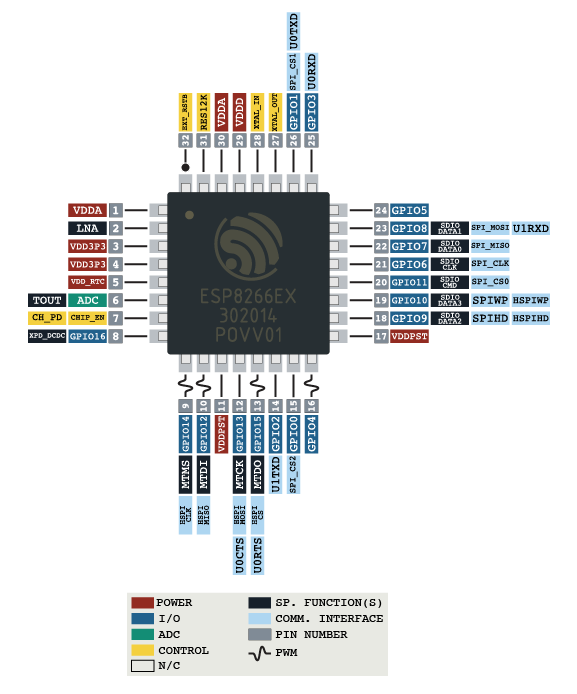
\includegraphics[scale=0.5]{analisis/esp8266_soc_pinout}
\caption{ESP8266EX SoC Pinout}
\label{fig:esp8266_soc_pinout}
\end{figure}

\begin{table}[!h]
\centering
\begin{tabular}{ |l|m{20em}| }
\hline
Voltaje de operación      & 2.5V $\sim$ 3.6V          \\ \hline
Consumo                   & 20 uA - 170 mA (80 mA avg.)  \\ \hline
Temperatura de operación  & -40°C $\sim$ 125°C        \\ \hline
Procesador                & Tensilica L106 32-bit     \\ \hline
Frecuencia de reloj       & 80 MHz / 160 MHz          \\ \hline
Interfaces                & UART, SDIO, SPI, I2C, I2S, IR Remote Control, GPIO, ADC y PWM                           \\ \hline
GPIO pins                 & 17                        \\ \hline
RAM (espacio de usuario)  & < 50 kB                     \\ \hline
Protocolos WiFi           & 802.11 b/g/n (HT20)       \\ \hline
Rango de frecuencias WiFi & 2.4G $\sim$ 2.5G (2400M $\sim$ 2483.5M) \\ \hline
\end{tabular}
\caption{Características ESP8266}
\label{table:caracteristicas_esp8266}
\end{table}

Debido a que el ESP8266 viene en un pequeño empaquetado (QFN-21) algunos fabricantes han desarrollado módulos (MCU) que facilitan su uso, proporcionando componentes necesarios para el desarrollo como son la memoria flash externa y pines externos para GPIO.\\

Espressif dispone de sus propio módulos, la serie ESP-WROOM-02 \cite{espwroom02_overview}, el módulo base \cite{espwroom02_datasheet} lleva el mismo nombre que la serie y tiene un tamaño de 18 mm x 20 mm e integran una memoria flash SPI de 2 MB y una antena PCB, además dispone de 18 pines (Figura \ref{fig:esp01_pinout}). Existen otros modelos de la serie con 4MB de memoria flash y con conectores IPEX para una antena externa en lugar de la antena PCB. El precio medio de esta serie es de 2,50€ \cite{espressif_provider_digikey} \cite{espressif_provider_mouser}\\

\begin{figure}[h]
\centering
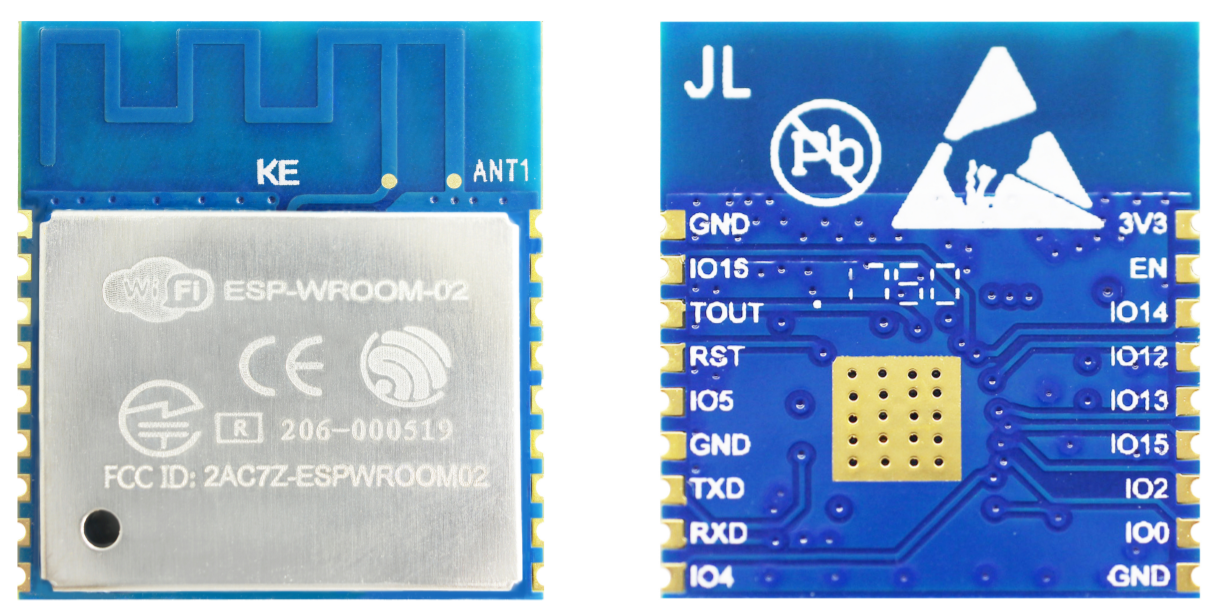
\includegraphics[scale=0.2]{analisis/esp_wroom_02}
\caption{Módulo ESP-WROOM-02}
\label{fig:esp_wrom_02}
\end{figure}

A pesar de que el fabricante original del ESP8266, Espressif, dispone de sus propios módulos, este SoC empezó realmente a popularizarse en el 2014 con el módulo ESP-01 creado por un tercer fabricante, Ai-Thinker. El módulo añade una memoria flash externa QSPI, una antena impresa en la PCB y proporciona salida para algunos de los pines del ESP8266 (Figura \ref{fig:esp01_pinout}).\\

\begin{figure}[H]
\centering
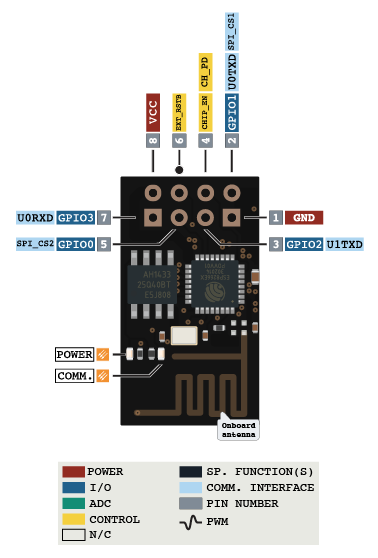
\includegraphics[scale=0.5]{analisis/esp01_pinout}
\caption{ESP-01 Pinout}
\label{fig:esp01_pinout}
\end{figure}

Desde este primer modelo se han desarrollado multitud de modelos con variaciones respecto al número de pines expuestos, tipo de antena y memoria flash; pero manteniendo el mismo SoC ESP8266EX. Se les conoce como módulos ESP-XX y la última versión es el ESP-14 que combina en el mismo encapsulado el SoC ESP8266EX junto con un microcontrolador STMicro STMS003F3P6. Aunque el modelo más utilizado de esta serie es el ESP-12 y sus variantes con apantallamiento y un mayor número de conexiones, en concreto 22, a excepción del módulo ESP-12S que cuenta con 16. (Figura \ref{fig:esp12e_pinout}).\\

\begin{figure}[H]
\centering
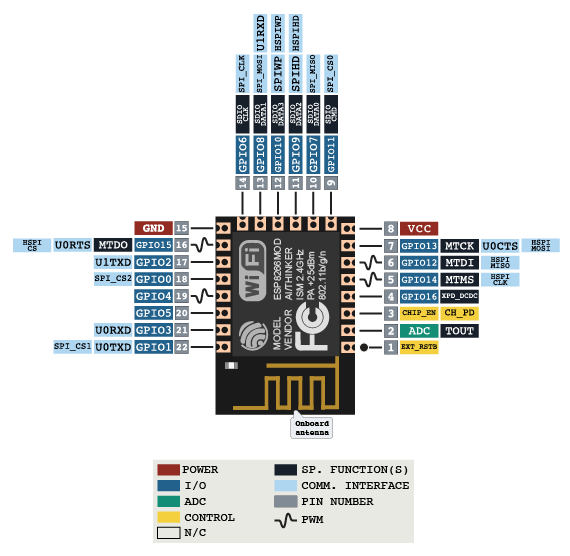
\includegraphics[scale=0.5]{analisis/esp12e_pinout}
\caption{ESP-12E Pinout}
\label{fig:esp12e_pinout}
\end{figure}

Aunque estos módulos son más cómodos seguimos teniendo la necesidad de adquirir un adaptador USB-Serial y un regulador de voltaje y cablearlos al módulo para poder programarlo.Para suplir estas necesidades nacieron los módulos de desarrollo (Devkits), estos módulos están enfocados al desarrollo y a facilitar la creación de prototipos, para ello incluyen un puente USB-Serial integrado en la placa y un conector micro-USB junto con un regulador de voltaje para proporcionar energía a la placa y conectividad con el ordenador, además de otras facilidades como botones, leds o conectores para baterías y antenas.\\

Algunos modelos están basado en módulos ESP-XX de Espressif como el Adafruit Feather HUZZAH \cite{adafruit_feather_huzzah} que utiliza un módulo Ai-Thinker ESP-12S, en la figura \ref{fig:adafruit_feather_huzzah_pinout_2} se pude apreciar como el módulo de Ai-thinker está soldado directamente encima de la placa de desarrollo.\\~\\

\begin{figure}[H]
\centering
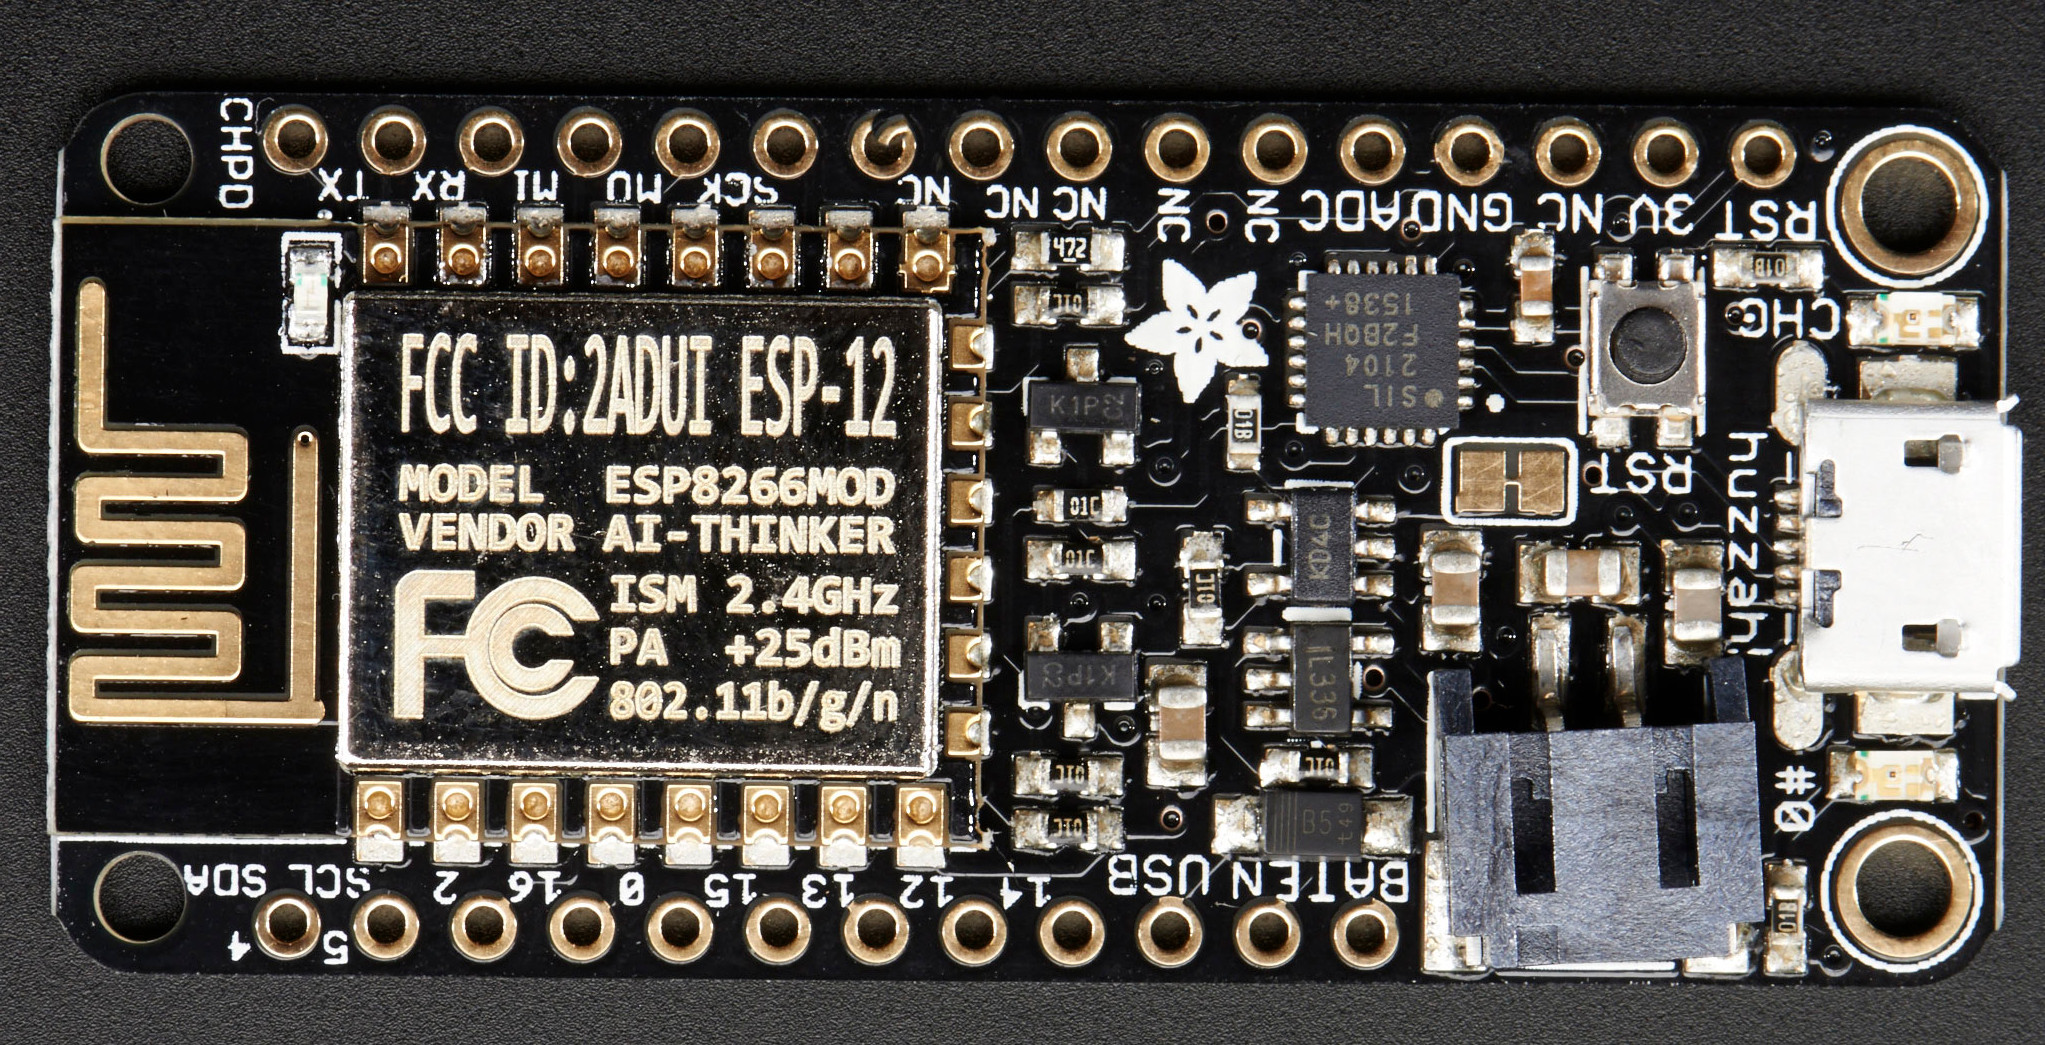
\includegraphics[scale=0.12]{analisis/adafruit_feather_huzzah_pinout_2}
\caption{Adafruit Feather HUZZAH}
\label{fig:adafruit_feather_huzzah_pinout_2}
\end{figure}

Otros módulos de desarrollo no usan un módulo intermediario, en su lugar incorporan directamente el chip en la placa como es el caso del WEMOS D1 Mini Pro \cite{wemos_d1_mini_pro} que utiliza un ESP8266EX (Figura \ref{fig:wemos_d1_mini_pro}).\\

\begin{figure}[h]
\centering
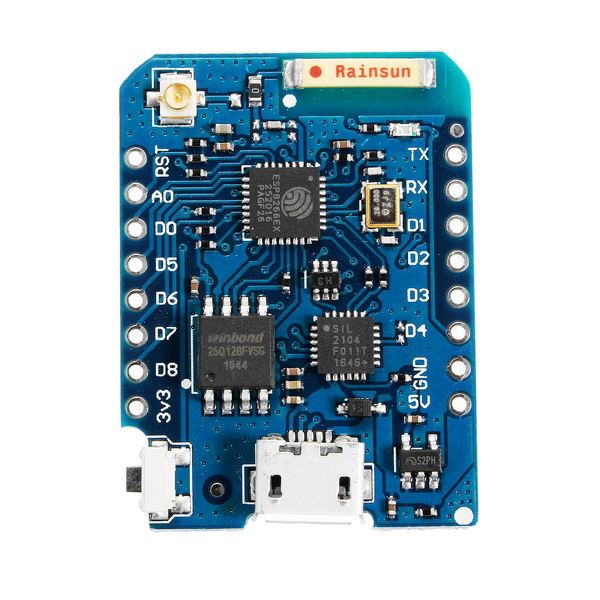
\includegraphics[scale=0.5]{analisis/wemos_d1_mini_pro}
\caption{WEMOS D1 Mini Pro}
\label{fig:wemos_d1_mini_pro}
%https://wiki.wemos.cc/products:retired:d1_mini_pro_v1.1.0
\end{figure}

Existen una gran variedad de estos módulos de diferentes fabricantes, algunos de los más conocidos son:  Feather de la empresa Adafruit Industries, ESP8266 Thing de la empresa SparkFun Electronics y NodeMCU del fabricante Lolin. Hay un gran rango de precios desde los 3€ del modelo de WEMOS a los 15€ del modelo de SparkFun \cite{espressif_provider_digikey} \cite{espressif_provider_mouser}\cite{sparkfun_thing_official_page}.\\


\noindent{\textbf{ESP32}}\\
El ESP32, es una familias de SoC's de bajo coste y consumo con WiFi y Bluetooth modo dual integrado, también diseñado por Espressif Systems \cite{esp32_overview} es el sucesor del ESP8266.\\

La familia de SoCs ESP32 dispone de una gran variedad de modelos la mayoría en un formato QFN de 5x5 mm y 6x6 mm (Figura \ref{fig:esp32_soc_pinout}) a excepción de la familia PICO que usan un encapsulado LGA de 7x7 mm, todos los modelos tienen 48 pines y utilizan microprocesadores Xtensa 32-bit LX6 en versiones de un solo núcleo dos dependiendo del modelo, ambas versiones pueden trabajar en frecuencias desde 80 MHz hasta 240MHz. Al desarrollar estos nuevos SoCs Espressif les doto de características ideales para dispositivos wearables como el soporte para BLE, sensores táctiles capacitivos o modo de sueño para ahorro energético con el que consume menos de 5  uA. El precio de estos SoCs oscila entre 0,89€ y 3€ en los distribuidores oficiales de Espressif \cite{espressif_provider_digikey} \cite{espressif_provider_mouser}.\\

\begin{figure}[H]
\centering
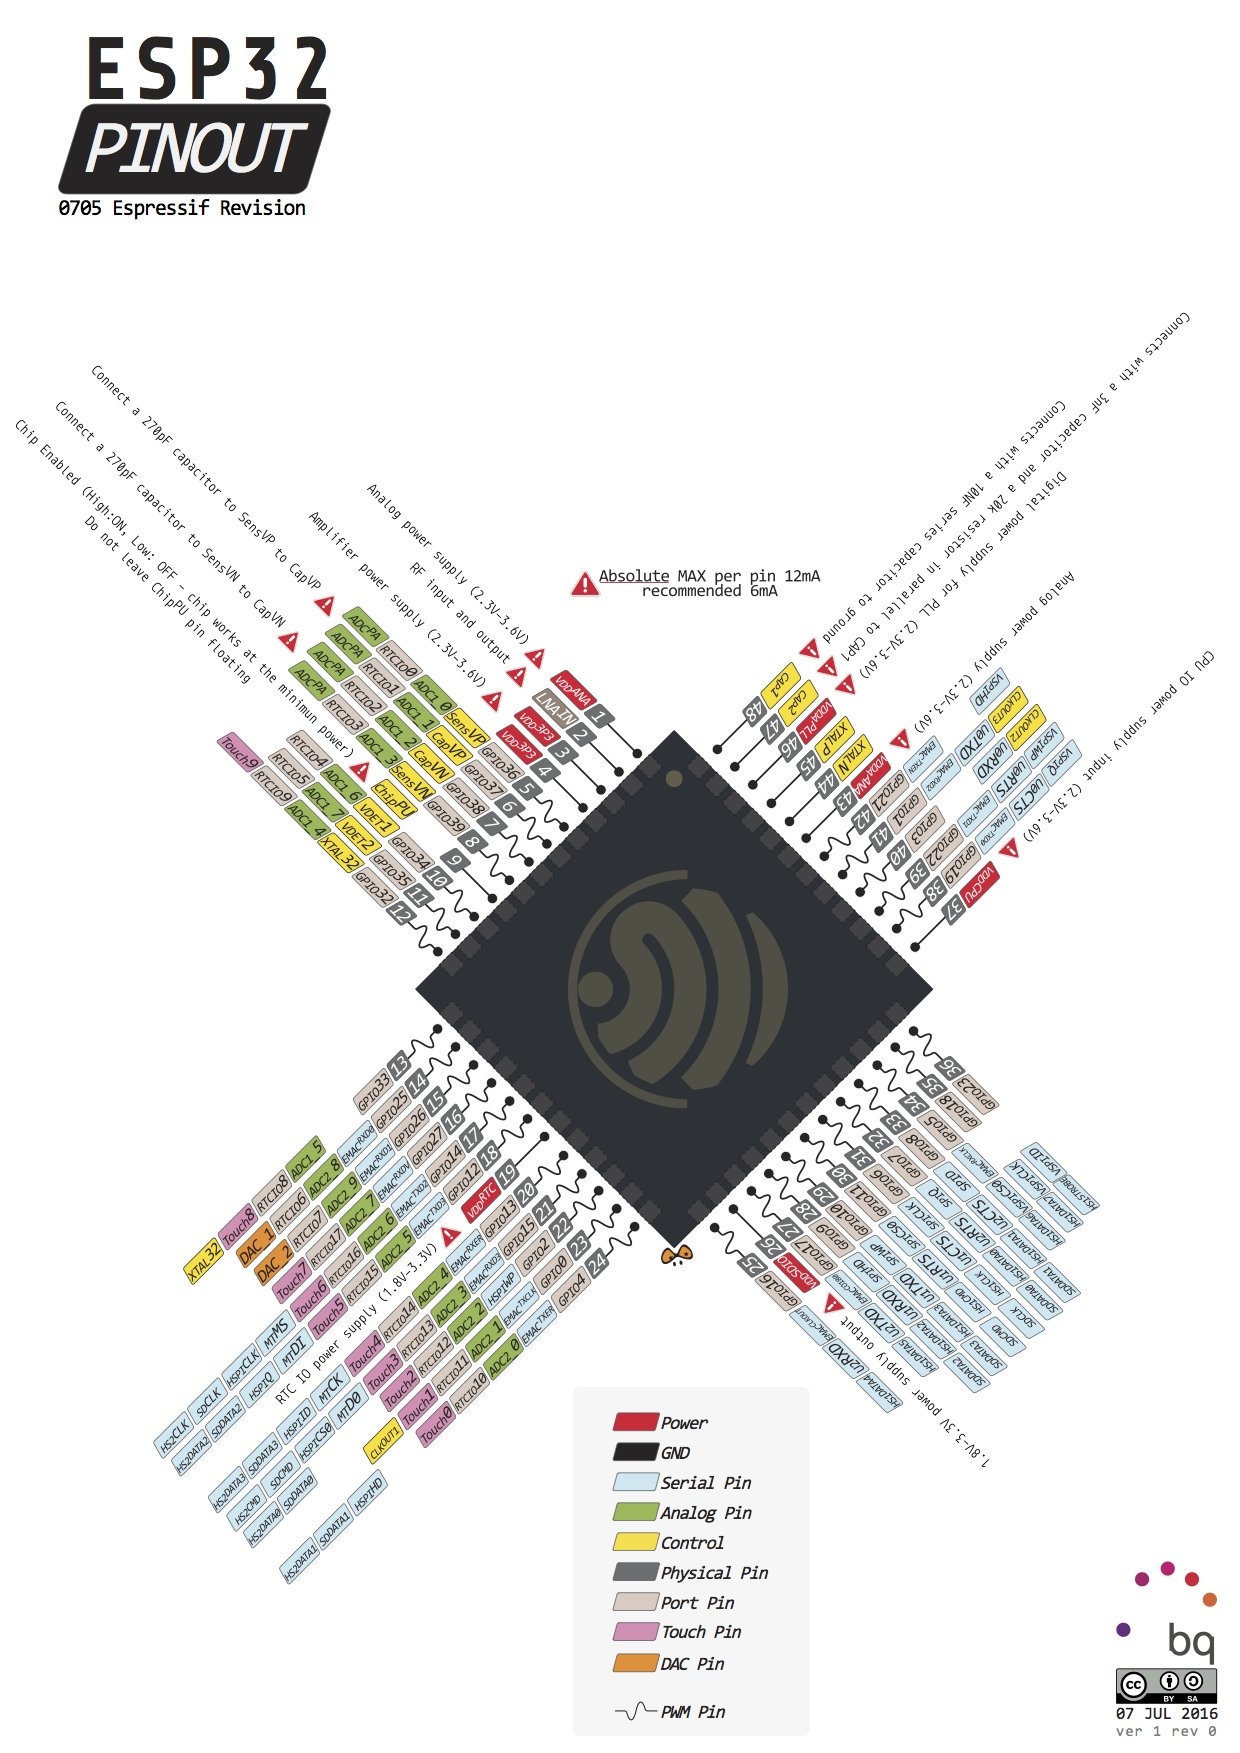
\includegraphics[scale=0.3]{analisis/esp32_soc_pinout}
\caption{ESP32 SoC Pinout  \cite{esp32_soc_pinout}.}
\label{fig:esp32_soc_pinout}
\end{figure}

\begin{table}[h!]
\centering
\begin{tabular}{ |l|m{20em}| }
\hline
Voltaje de operación      & 2.3V $\sim$ 3.6V          \\ \hline
Consumo                   & 10 uA - 68 mA  \\ \hline
Temperatura de operación  & -40°C $\sim$ 125°C        \\ \hline
Procesador                & Xtensa single-/dual-core 32-bit LX6 microprocessor(s)   \\ \hline
Frecuencia de reloj       & 80 MHz / 160 MHz  / 240 MHz        \\ \hline
Interfaces                & 3 x UART, SDIO, 4 x SPI, 2 x I2C, 2 x I2S, IR, 12-bit SAR ADC, 2 x 8-bit DAC, CAN 2.0, 10 x touch sensors, SD card interface, Ethernet y PWM                           \\ \hline
GPIO pins                 & 34                        \\ \hline
RAM (espacio de usuario)  & < 50 kB                     \\ \hline
Protocolos WiFi           & 802.11 b/g/n (HT20)       \\ \hline
Rango de frecuencias WiFi & 2.4G $\sim$ 2.5G (2400M $\sim$ 2483.5M) \\ \hline
Bluetooth           &  Bluetooth v4.2 BR/EDR y BLE dual-mode  \\ \hline
\end{tabular}
\caption{Características ESP32}
\label{table:caracteristicas_esp32}
\end{table}

Al igual que su predecesor se comercializa en tres formatos: SoC, módulos y DevKits. Esta vez Espressif aposto desde el principio por comercializar sus propios módulos y desarrollo una gran variedad de módulos, actualmente comercializa 13 variantes agrupadas en tres familias: ESP32-SOLO, ESP32-WROOM y ESP32-WROVER \cite{espressif_products_ordering_information}. La familia SOLO integra SoCs de un solo núcleo mientras las familias WROOM y WROVER utilizan doble núcleo, además esta última tiene memoria SPIRAM ideal para aplicaciones que requieren más memoria como productos AIoT. Con unas dimensiones que van desde los 18.00×25.50×3.10 mm hasta los 18.00×31.40×3.30 mm estos módulos contienen una memoria flash (4, 8 y 16 MB) y antena impresa PCB o conector IPEX para poder conectar antenas de mayor potencia. El precio de estos módulos oscila entre los 1,80€ hasta los 4,50€ dependiendo del modelo \cite{espressif_provider_digikey} \cite{espressif_provider_mouser}.\\

\begin{figure}[H]
\centering
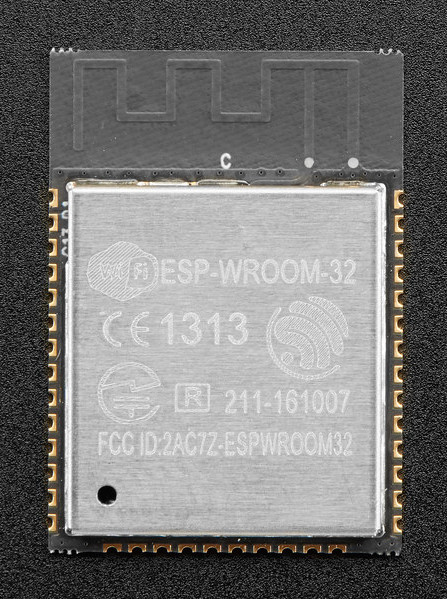
\includegraphics[scale=0.2]{analisis/esp32_module}
\caption{Módulo ESP32  \cite{esp32_module}.}
\label{fig:esp32_module}
\end{figure}

Espressif también ofrece una gran variedad de DevKits para todo tipo de aplicaciones, desde placas con pantalla táctil integrada como la ESP32-S2-Kaluga-1, la ESP-EYE con cámara integrada para reconocimiento de imágenes e incluso placas con micrófonos, tecnologías de cancelación de ruido incorporadas y soporte para conectar con los servicios de asistente de voz de Google y Amazon como las ESP32-LyraTD. El modelo más básico, ESP32-DevKitC, se puede adquirir por aproximadamente 9€ en los distribuidores oficiales \cite{espressif_provider_digikey} \cite{espressif_provider_mouser}.\\

\begin{figure}[H]
\centering
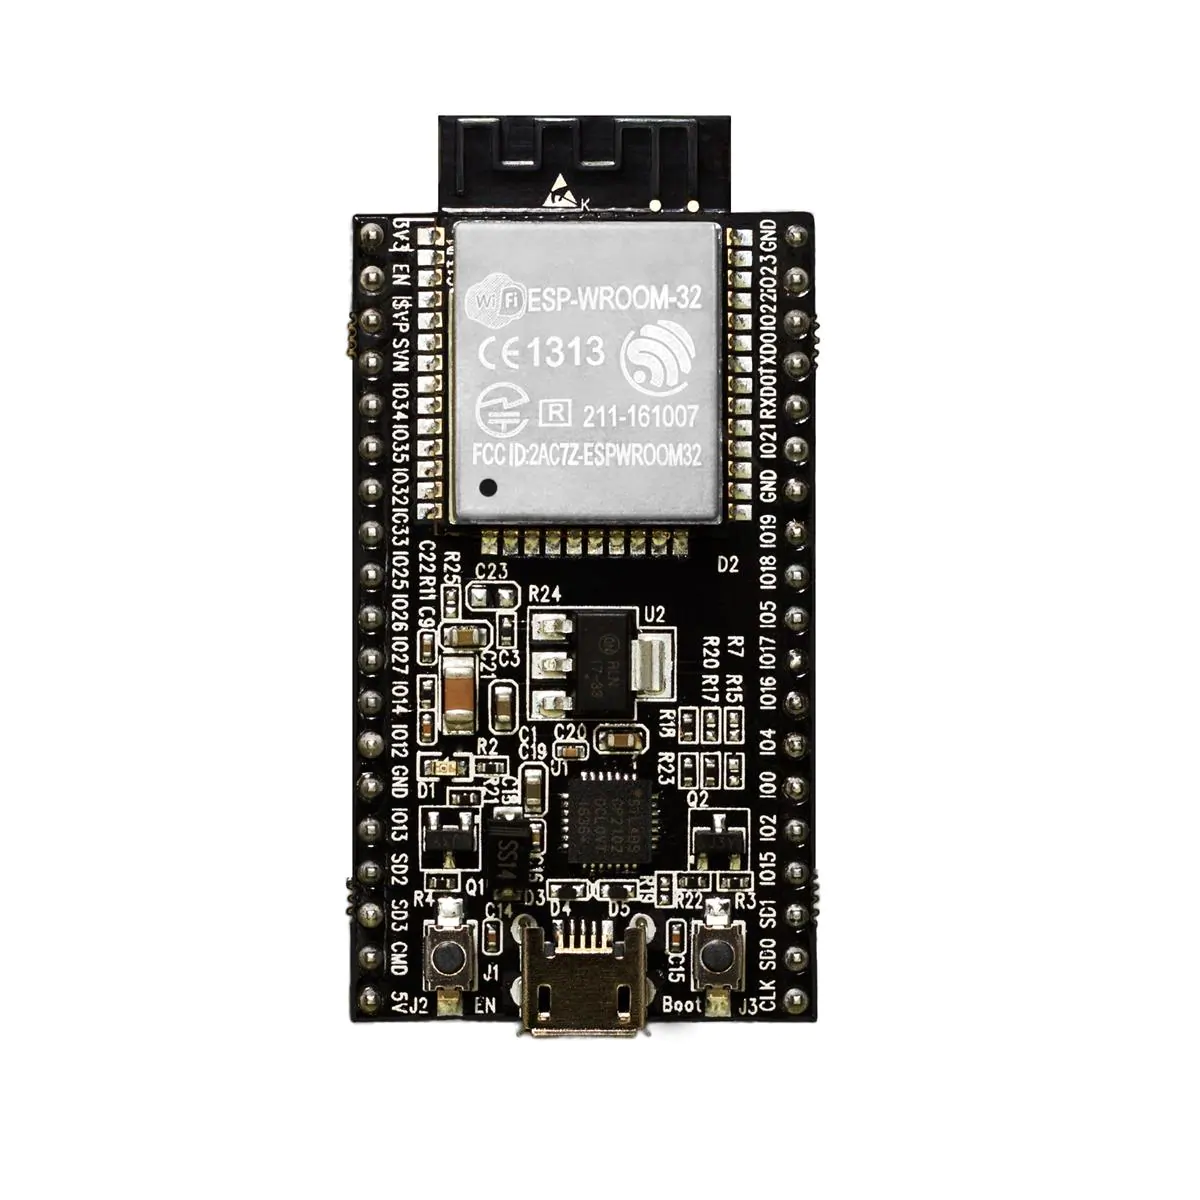
\includegraphics[scale=0.2]{analisis/esp32_devkitc_32u}
\caption{Módulo de desarrollo ESP32-DevKitC-21U.}
\label{fig:esp32_devkitc_32u}
\end{figure}

\noindent{\textbf{Elección}}\\

Para el desarrollo de este proyecto se han utilizado módulos de desarrollo ya que facilitan un desarrollo rápido y cómodo al permitir programar y alimentar el módulo fácilmente a través de una conexión USB, aunque no es habitual utilizar este tipo de módulos en aplicaciones reales ya que encarecería el coste del despliegue al incluir componentes que no serían necesarios una vez desplegados, por ejemplo, no es necesario que los dispositivos ya desplegados incluyan un adaptador USB-Serial ya que normalmente solo serán programados inicialmente y en caso de ser necesario actualizarlos se podría usar un adaptador externo o realizar actualizaciones vía OTA. Una vez completado el desarrollo lo normal es utilizar módulos como el ESP-12 o un ESP32-WROOM con un menor tamaño y consumo, aunque si no es un despliegue de grandes magnitudes, por ejemplo, para realizar investigaciones usar un módulo de desarrollo podría seguir siendo una buena opción ya que ahorraría crear el diseñó de la placa de alimentación que necesitaría un módulo.

Para el desarrollo de este proyecto en un principio se eligió el módulo de desarrollo WEMOS D1 Mini Pro basado en el SoC ESP8266, con unas dimensiones de 34.2 mm x 25.6 mm y un peso de 3 g es una de las placas más pequeñas del mercado, con un tamaño ligeramente más grande que un módulo ESP-12 (24.0 mm × 16.0 mm) incorpora un conversor P2104 USB-TO-UART, antena cerámica incorporada memoria flash de 16 MB y un regulador de tensión que permite alimentarlo a 5 V a través de un micro-USB. Una de los principales motivos para la elección de este módulo de desarrollo fue su reducido tamaño, la posibilidad de conectar una antena externa para mejorar el alcance mediante un conector de tipo U.FL y su reducido precio de tan solo 3€ \cite{lolin_official_store}. \\

Otra de las ventajas de este módulo de desarrollo, a pesar de estar fuera del alcance de este proyecto, es la posibilidad de ampliar la funcionalidad a través de la conexión de expansiones en formato shields. Existe una gran variedad shields como, por ejemplo, pantalla oled, relé o controlador de motores (Figura \ref{fig:wemos_d1_mini_shields}).\\

\begin{figure}[H]
\centering
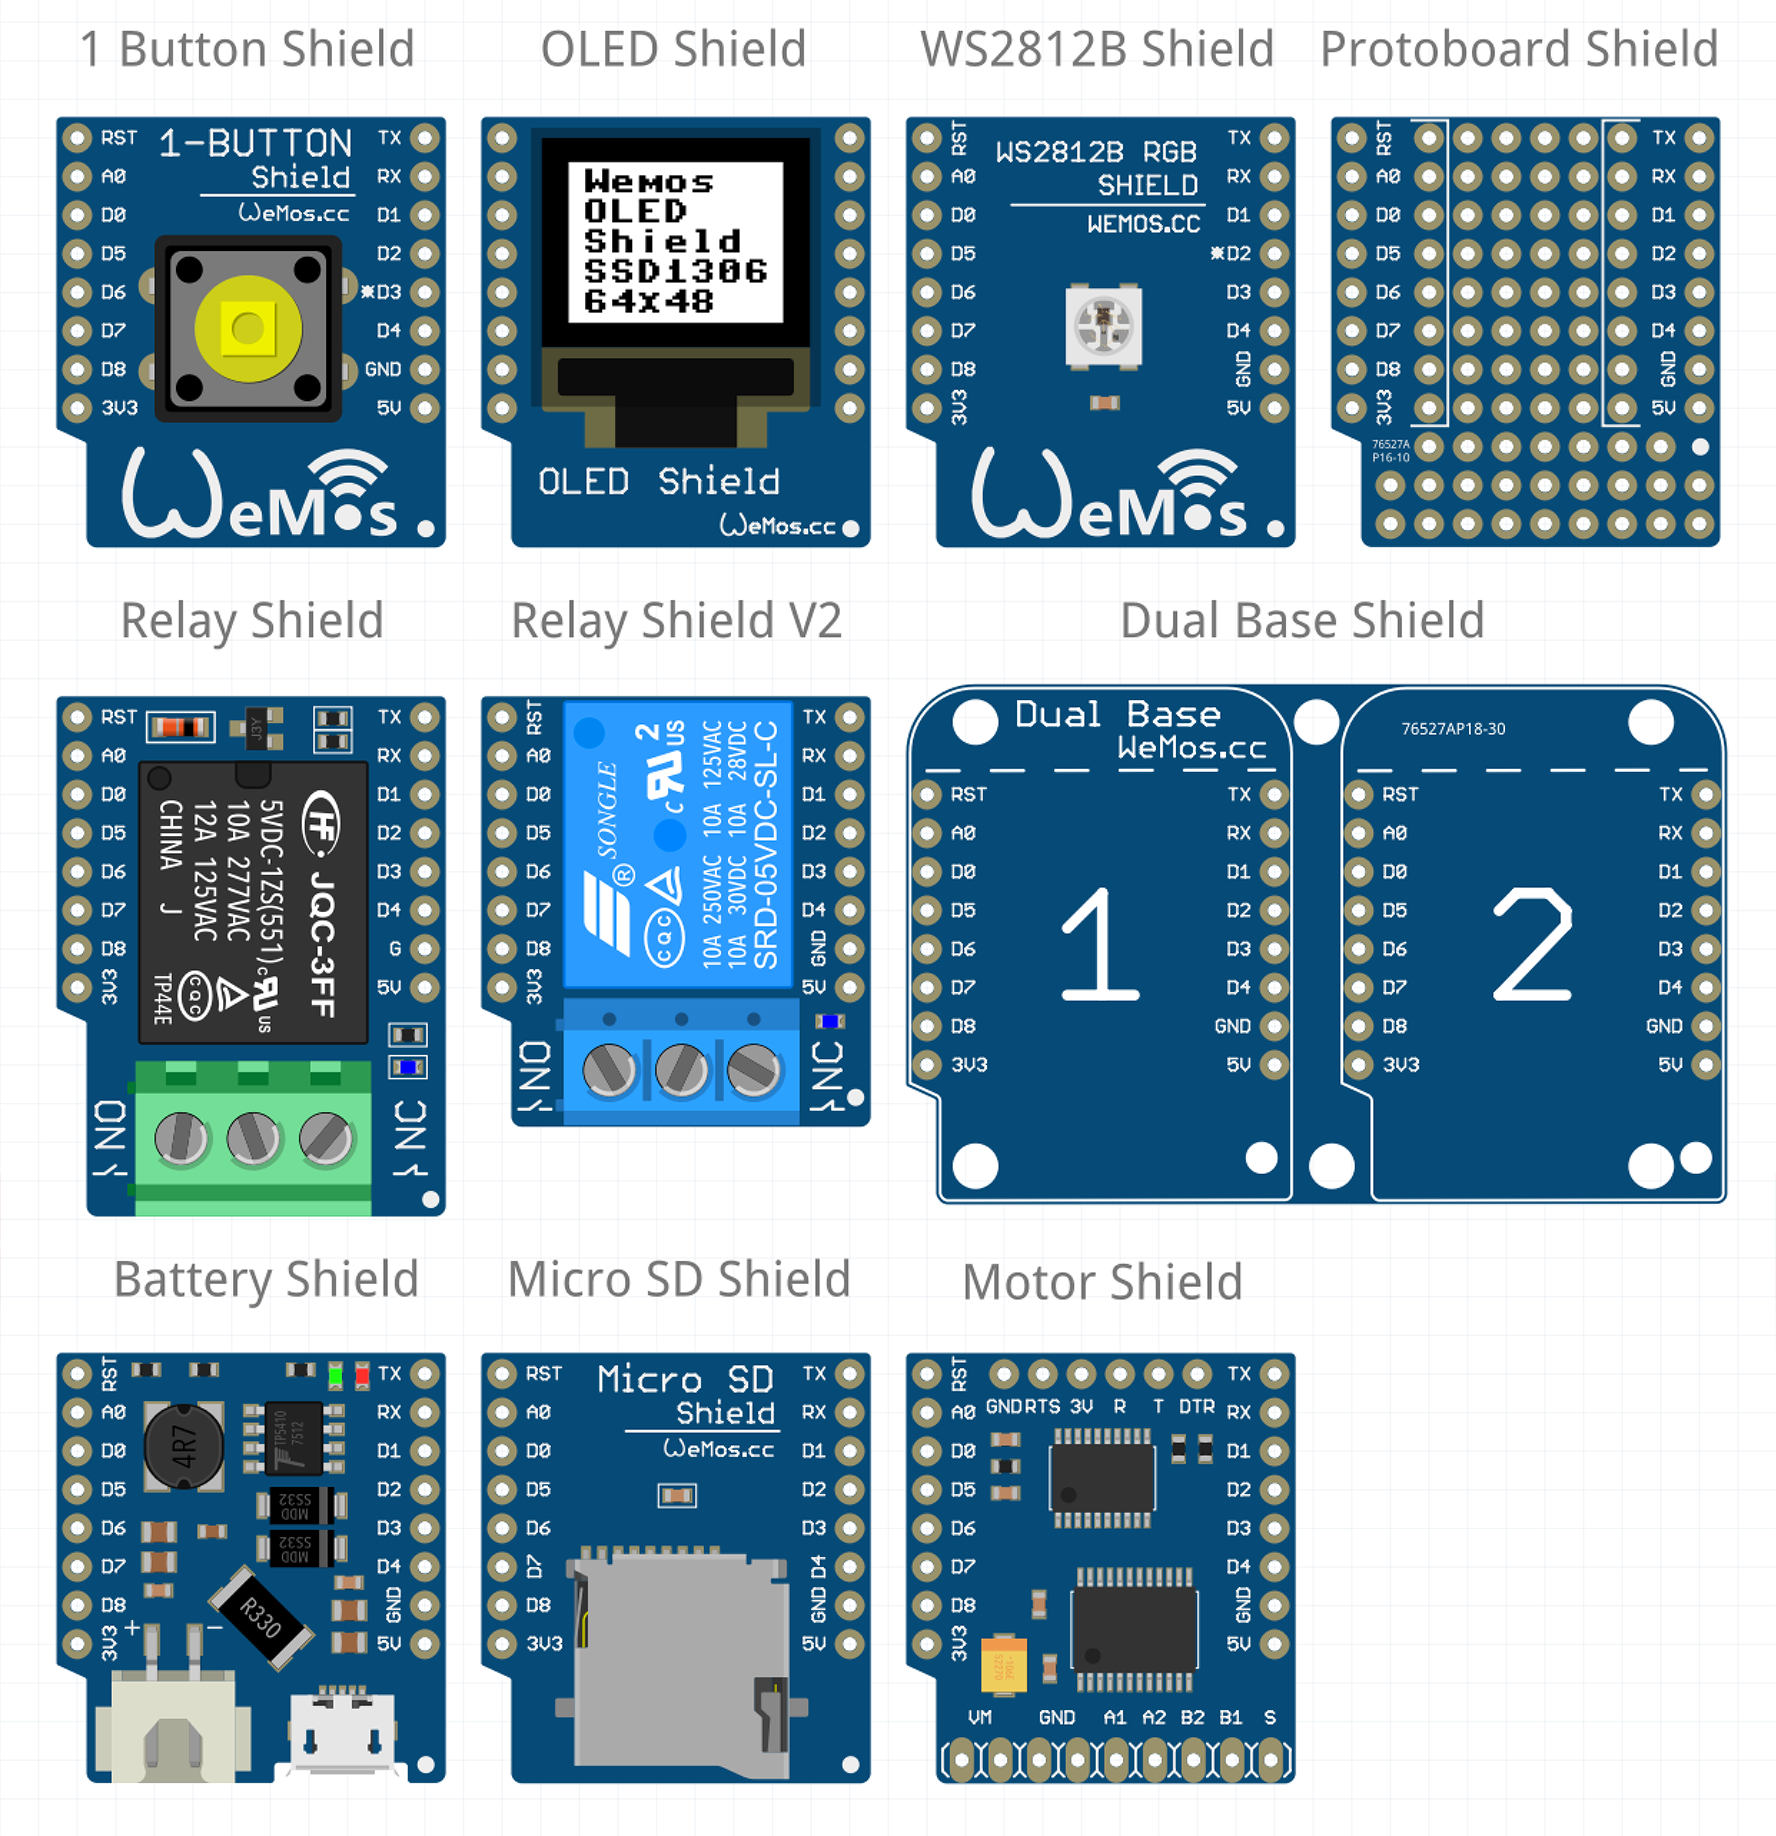
\includegraphics[scale=0.15]{analisis/wemos_d1_mini_shields}
\caption{WEMOS D1 Mini Shields}
\label{fig:wemos_d1_mini_shields}
%https://github.com/mcauser/Fritzing-Part-WeMos-D1-mini-Shields
\end{figure}

Como punto negativo este módulo no cuenta con Bluetooth integrado por lo que para cumplir los requisitos de este proyecto es necesario usarlo junto a un módulo Bluetooth externo como el HC-05 (Figura \ref{fig:hc05_bluetooth_module}), estos módulos se pueden conectarse fácilmente con el ESP8266 usando el puerto serie y se configuran utilizando comandos AT, se pueden adquirir por alrededor de 2€ por lo que el coste total en componentes sería de aproximadamente unos 5€ por lo que seguiría cumpliendo el requisito del bajo coste.

\begin{figure}[H]
\centering
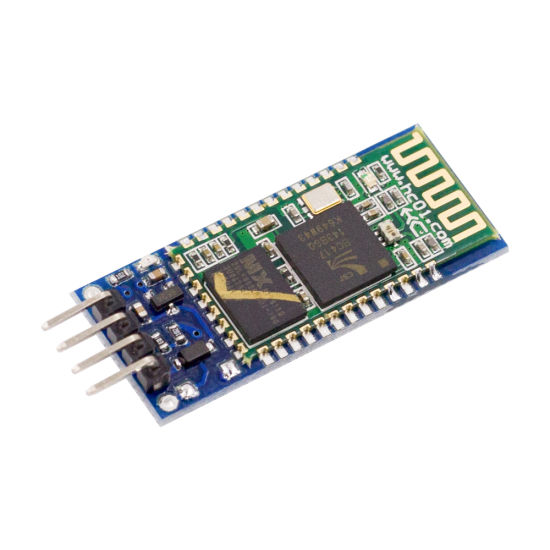
\includegraphics[scale=0.2]{analisis/hc05_bluetooth_module}
\caption{Módulo Bluetooth HC-05}
\label{fig:hc05_bluetooth_module}
%https://github.com/mcauser/Fritzing-Part-WeMos-D1-mini-Shields
\end{figure}

Por las razones expuestas inicialmente se decidió utilizar el SoC ESP8266 junto con el módulo Bluetooth HC-05 ya que cumplía con el requisito del bajo coste mejor que ninguna de las opciones incluso teniendo en cuenta el hecho de tener que adquirir el módulo Bluetooth por separado, pero durante el desarrollo del proyecto se apreció que en la valoración inicial no se había tenido en cuenta el coste que supondría el proceso de integración de estos módulo, aunque aparentemente una operación sencilla como es el soldado o cableado de estos dos módulos supondría un gran coste en mano de obra para realizar grandes despliegues. Este motivo llevo a replantear la opción del ESP32 ya que este SoC dispone de conectividad Bluetooth nativa, inicialmente fue descartado por tener un mayor coste pero al tener en cuenta los costes de integración de la primera elección quedan igualados en este punto, también simplificaría el diseño al poder configurar el Bluetooth sin necesidad de utilizar comandos AT, además dispone de un procesador más potente y de doble núcleo. Por todo lo expuesto finalmente se eligió el SoC ESP32 como solución para este proyecto.\\

\section{Framework}

Actualmente existen multitud de \textit{frameworks} de desarrollo para el SoC ESP32, basados en una gran variedad de lenguajes como: C, C++, Python, JavaScript o Lua. A continuación se analizan algunos de los  \textit{frameworks} más usados.\\

\noindent{\textbf{Espressif IoT Development Framework (ESP-IDF)}}\\
ESP-IDF es el \textit{framework} de desarrollo oficial creado por Espressif Systems para el SoC ESP32. Está escrito principalmente en C  y está basado en el sistema operativo en tiempo real FreeRTOS. Es uno de los más usados y tiene una gran comunidad siendo fácil encontrar ayuda en sus foros oficiales, además cuenta con una extensa documentación oficial. La mayoría de \textit{frameworks} que trabajan sobre C o C++ están construidos sobre la API de ESP-IDF. Para trabajar con el solo es necesaria la toolchain propia, algunas herramientas de construcción (CMake y Ninja) y por supuesto el propio paquete ESP-IDF que contiene la API y algunos scripts para facilitar el uso de la toolchain. Con estas herramientas y un simple editor de texto ya podríamos empezar a crear aplicaciones para el ESP32 aunque es recomendable utilizar algún IDE como PlatformIO IDE.\\

 Las principales ventajas de este \textit{framework} es que al ser el oficial del fabricante es en el que primero obtendremos nuevas funcionalidades y parches de seguridad, otra de sus ventajas es que al tener un menor nivel de abstracción que permite un acceso a más bajo nivel que el resto, esto a su vez es su desventaja ya resulta en un código más extenso, a continuación podemos ver un ejemplo de un código para hacer parpadear un led.\\

\begin{minipage}{\linewidth}
\begin{lstlisting}[language=C, caption=Ejemplo de código para hacer parpadear un led con ESP-IDF, captionpos=b, frame=single]
#include <stdio.h>
#include "freertos/FreeRTOS.h"
#include "freertos/task.h"
#include "driver/gpio.h"
#include "sdkconfig.h"

#define BLINK_GPIO CONFIG_BLINK_GPIO

void app_main(void)
{
    gpio_reset_pin(BLINK_GPIO);
    gpio_set_direction(BLINK_GPIO, GPIO_MODE_OUTPUT);
    while(1) {
        gpio_set_level(BLINK_GPIO, 0);
        vTaskDelay(1000 / portTICK_PERIOD_MS);
        gpio_set_level(BLINK_GPIO, 1);
        vTaskDelay(1000 / portTICK_PERIOD_MS);
    }
}
\end{lstlisting}
\end{minipage}

\noindent{\textbf{Arduino}}\\
Arduino es una plataforma de código abierto utilizada para la construcción de proyectos de electrónica, dentro de está plataforma encontramos el lenguaje de programación Arduino y el entorno de desarrollo IDE. Arduino es un lenguaje potente y sencillo que permite desarrollar proyectos en C/C++ sin requerir grandes conocimientos de electrónica. Gracias a su espíritu de código abierto ha crecido una gran comunidad a su alrededor que ha contribuido creando todo tipo de librerías y herramientas.\\

Este lenguaje fue inicialmente diseñados para utilizar sobre las placas Arduino pero con su creciente popularidad se han realizado multitud de adaptaciones para usarlo en otros microcontroladores como es el caso del ESP32, esta adaptación esta basada en ESP-IDF y fue realizada por el propio fabricante del SoC Espressif Systems, nos permite un mayor nivel de abstracción y acceso a una gran cantidad de librerías sin perder acceso a funcionalidades a más bajo nivel usando funciones del ESP-IDF ya que las librerías están integradas en la compilación de la librería de Arduino.\\

Resumiendo, sus principales ventajas son el nivel de abstracción y su comunidad, otra de sus ventajas es el entorno de desarrollo Arduino IDE que nos permite realizar de forma sencilla acciones como compilar o subir el código a la plac, tambiés posible utilizarlo con el IDE de PlatformIO, ambos disponen de un gestor de librerías que nos permite buscar e instalarlas fácilmente. Como desventaja el tener un mayor nivel de abstracción siempre implica perder algo de control.\\

\begin{minipage}{\linewidth}
\begin{lstlisting}[language=C, caption=Ejemplo de código para hacer parpadear un led con Arduino, captionpos=b, frame=single]
const int LED_BUILTIN = 2;
void setup() {
  pinMode (LED_BUILTIN, OUTPUT);
}
void loop() {
  digitalWrite(LED_BUILTIN, HIGH);
  delay(1000);
  digitalWrite(LED_BUILTIN, LOW);
  delay(1000);
}
\end{lstlisting}
\end{minipage}

\noindent{\textbf{MicroPython}}\\
MicroPython es una implementación del lenguaje de programación Python 3 que incluye una pequeño subconjunto de la biblioteca estándar de Python y está optimizada para ejecutarse en microcontroladores. Originalmente fue diseñado para ejecutarse sobre la placa PyBoard pero actualmente se ha adaptado a un amplio número de arquitecturas. No dispone de un IDE propio pero hay varias alternativas como uPyCraft, Thonny o  VSCode con la extensión PyMark.\\

Su principal ventaja además de portar la simplicidad del lenguaje Python al mundo de los microcontroladores es que una vez cargado en la placa podemos ejecutar comandos en el ESP32 directamente a través del serial como si fuera una consola python normal y corriente, esto agiliza mucho el proceso de desarrollo ya que nos permite realizar pruebas sin tiempos de compilación ni de subida a la placa. Su mayor desventaja es que no permite acceder  a funciones a bajo nivel por ejemplo para las funcionalidades WiFi y no dispone de tantas librerías como las anteriores opciones.\\

\begin{minipage}{\linewidth}
\begin{lstlisting}[language=Python, caption=Ejemplo de código para hacer parpadear un led con MicroPython, captionpos=b, frame=single]
from machine import Pin
import time import sleep

led=Pin(2, Pin.OUT)

while True:
  led.value(not led.value())
  time.sleep(1)
\end{lstlisting}
\end{minipage}

\noindent{\textbf{NodeMCU}}\\
NodeMCU es una plataforma de código abierto que incluye tanto el firmware basado en LUA como un módulo de desarrollo homónimo basado en los SoCs de Espressif, el lenguaje inicialmente se desarrolló para las placas NodeMCU pero ahora se puede ejecutar en cualquier módulo ESP.\\

Su principal característica es que usa un modelo de programación similar a Node.js basado en la  asincronía  y en arquitectura dirigida por eventos, la mayoría de sus funciones tienen un parámetro para funciones \textit{callback}. Como desventaja LUA no es un lenguaje muy popular por lo que normalmente requerirá que el desarrollador tenga que aprender un nuevo lenguaje desde cero, además no dispone de un IDE por lo que empezar a trabajar con el no es tan sencillo como en el resto de opciones.\\

\begin{minipage}{\linewidth}
\begin{lstlisting}[language={[5.0]Lua}, caption=Ejemplo de código para hacer parpadear un led con NodeMCU, captionpos=b, frame=single]
lighton=0
tmr.alarm(0,1000,1,function()
if lighton==0 then
    lighton=1
    led(512,512,512)
    -- 512/1024, 50% duty cycle
else
    lighton=0
    led(0,0,0)
end
end)
\end{lstlisting}
\end{minipage}

\noindent{\textbf{Mongoose OS}}\\
Mongoose OS es una plataforma de desarrollo de código abierto enfocada a la integración con las plataformas cloud IoT como Amazon, Azureo Google, también dispone de una versión empresarial con licencia comercial que dispone de más funcionalidades la versión libre. Su propósito es ser un entorno completo para la creación de prototipos, desarrollo y gestión de dispositivos conectados.\\

Una de sus principales ventajas es que permite programar tanto en JavaScript como en C, además dispone de un IDE muy completo con interfaz web. Su principal desventaja es que algunas librerías son de código cerrado y es necesario adquirir una licencia para poder utilizarlas. También cabe destacar que aunque la opción de programar con JS pueda resultar atractiva para un prototipado rápido durante el desarrollo no es recomendable usarlo en producción ya que tiene una mayor sobrecarga en consumo de memoria y CPU.\\


\begin{minipage}{\linewidth}
\begin{lstlisting}[caption=Ejemplo de código para hacer parpadear un led con Moongose, captionpos=b, frame=single]
load('api_gpio.js');
load('api_timer.js');

let PIN = 2;

GPIO.set_mode(PIN, GPIO.MODE_OUTPUT);
GPIO.blink(pin, 1000, 1000);
\end{lstlisting}
\end{minipage}

\noindent{\textbf{Elección}}\\

Tras analizar los \textit{frameworks} expuestos anteriormente se optó por elegir Arduino como solución para este proyecto, las razones para esta elección han sido su gran facilidad de uso  y sencillez, dispone de una gran comunidad y trayectoria por lo que es muy fácil encontrar información y respuestas a cualquier duda, dispone de una gran cantidad de librerías que facilitaran el trabajo y además a pesar de su gran nivel de abstracción podemos seguir accediendo a bajo nivel gracias a la integración con ESP-IDF, requisito necesario en este proyecto dada la necesidad de utilizar las funciones de monitorización del tráfico WiFi no disponibles en la mayoría de \textit{frameworks}.

% [1]https://www.espressif.com/en/products/hardware/esp8266ex/overview
% [2]https://www.espressif.com/sites/default/files/documentation/0a-esp8266ex_datasheet_en.pdf
% [3]https://www.espressif.com/en/products/hardware/esp-wroom-02/overview


% FIGURAS
% [1] https://raw.githubusercontent.com/acrobotic/Ai_Docs/master/pinouts/esp8266_soc/esp8266_soc-01.png
% [2] ESP-01 Pinout https://github.com/acrobotic/Ai_Docs/blob/master/pinouts/esp8266_esp01/esp8266_esp01-01.png
\end{document}
